\begin{tikzpicture}
    \node at (0,0) {
    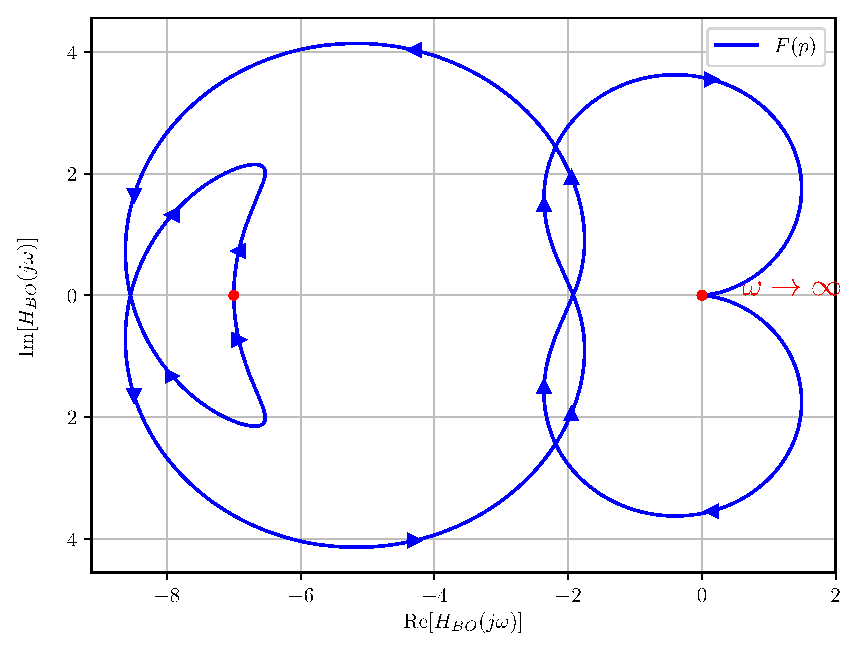
\includegraphics
    [width=0.8\textwidth]{fig/exercice_nyquist_chap_stab_ex1_enonce.eps}};
    \pgfmathsetmacro{\xu}{-4.32}
    \pgfmathsetmacro{\yu}{-0.05}
    \draw[red,fill=red] (\xu,\yu) circle (1.62pt) node[above left] {I$_1$};
    \pgfmathsetmacro{\xd}{-2.93}
    \pgfmathsetmacro{\yd}{-0.05}
    \draw[red,fill=red] (\xd,\yd) circle (1.62pt) node[above right] {I$_2$};
\end{tikzpicture}
